%%
% Please see https://bitbucket.org/rivanvx/beamer/wiki/Home for obtaining beamer.
%%
\documentclass[handout]{beamer}
% \mode<presentation> % change it to presentation model, but it does not work with [handout] option
\usepackage[T1]{fontenc}
\usepackage[utf8]{inputenc}
\usepackage{amsmath}
\usepackage{amssymb}
\usepackage{graphicx}
\usepackage{etoolbox} % adjust the space before and after figure
\usepackage{hyperref}
\usepackage{courier} % font for code in text
\usepackage{xeCJK} % Chinese 
\usepackage{listings}
\usepackage{wasysym}
\usepackage{amsthm} % for theorem definition style
\usepackage{rotating} % for the horizontal page table
\usepackage{pgfplots} % plot functions 

% \usepackage{enumitem} % never use this package for beamer

\usepackage{url}
\usepackage{natbib}
\usepackage{bm} % bold math symbol
\usepackage{blkarray}  % for labeling row and columns of matrix
\usepackage{tikz}
\usetikzlibrary{calc}
\usetikzlibrary{matrix}
\usetikzlibrary{positioning}
\usepackage{color}
\usepackage{setspace}
\usepackage{bm} % bold math symbol
\usepackage{bibentry}
\nobibliography*
\usepackage{listings}
\usepackage[export]{adjustbox}
\usepackage[ruled,vlined]{algorithm2e}  % algorithm 

\setbeamertemplate{caption}[numbered]  % set the figure number

% select the theme and color
\usetheme{Boadilla}
\usecolortheme{beaver}

\lstset{language=Python}
\definecolor{mygreen}{rgb}{0,0.6,0}
\definecolor{mygray}{rgb}{0.5,0.5,0.5}
\definecolor{mymauve}{rgb}{0.58,0,0.82}
\lstset{
  backgroundcolor=\color{white},   % choose the background color; you must add \usepackage{color} or \usepackage{xcolor}; should come as last argument
  basicstyle=\footnotesize,        % the size of the fonts that are used for the code
  breakatwhitespace=false,         % sets if automatic breaks should only happen at whitespace
  breaklines=true,                 % sets automatic line breaking
  captionpos=b,                    % sets the caption-position to bottom
  commentstyle=\color{mygreen},    % comment style
  deletekeywords={...},            % if you want to delete keywords from the given language
  escapeinside={\%*}{*)},          % if you want to add LaTeX within your code
  extendedchars=true,              % lets you use non-ASCII characters; for 8-bits encodings only, does not work with UTF-8
  frame=single,	                   % adds a frame around the code
  keepspaces=true,                 % keeps spaces in text, useful for keeping indentation of code (possibly needs columns=flexible)
  keywordstyle=\color{blue},       % keyword style
  language=Matlab,                 % the language of the code
  morekeywords={*,...},            % if you want to add more keywords to the set
  numbers=left,                    % where to put the line-numbers; possible values are (none, left, right)
  numbersep=5pt,                   % how far the line-numbers are from the code
  numberstyle=\tiny\color{mygray}, % the style that is used for the line-numbers
  rulecolor=\color{black},         % if not set, the frame-color may be changed on line-breaks within not-black text (e.g. comments (green here))
  showspaces=false,                % show spaces everywhere adding particular underscores; it overrides 'showstringspaces'
  showstringspaces=false,          % underline spaces within strings only
  showtabs=false,                  % show tabs within strings adding particular underscores
  stepnumber=2,                    % the step between two line-numbers. If it's 1, each line will be numbered
  stringstyle=\color{mymauve},     % string literal style
  tabsize=2,	                   % sets default tabsize to 2 spaces
  title=\lstname,                  % show the filename of files included with \lstinputlisting; also try caption instead of title
  belowcaptionskip= 1 ex,
  belowskip = 1 ex
}


\title[]{神经网络模型初探}
\subtitle{Introduction to Neural Network Model}

\date{\today}

\author[Michael]{王(云)斐, Michael}
\institute[SenseTime]{\url{https://www.michaelyunfei.com} \and \url{https://github.com/Michael-yunfei/MDLforBeginners}}

%[January 2019] (optional)
%{Demo for SenseTime}

\usecolortheme[RGB={128,0,0}]{structure}

\newcommand{\zn}{\mathbb{Z}}
\newcommand{\cn}{\mathbb{C}}
\newcommand{\qn}{\mathbb{Q}}
\newcommand{\rn}{\mathbb{R}}
\newcommand{\pn}{\mathbb{P}}
\newcommand{\fn}{\mathbb{F}}
\newcommand{\nn}{\mathbb{N}}


\begin{document}

\definecolor{franceblue}{RGB}{14, 76, 96}
\definecolor{brightred}{RGB}{243, 66, 53}



\begin{frame}[noframenumbering]
  \titlepage
\end{frame}



\begin{frame}{本节内容}
	\tableofcontents
\end{frame}

\section{课程设置简介}

\begin{frame}{课程进度和相关考核}
第三章内容跨度较大,我们分拆成两章来进行:
\begin{itemize}
\setlength\itemsep{1em}
	\item 辅导教义的第三章为本节课的讲解内容(教材44-56页)
	\item 辅导教义的第四章为下周教授的内容(教材第3章余下内容)
\end{itemize}

\hfil

辅导讲义的组成部分:
\begin{itemize}
\setlength\itemsep{1em}
	\item 课前预习C1
	\item 课堂讲义C2
	\item 课后练习C3
\end{itemize}

\hfil 

认真完成以上三个内容可以得到A, 只完成C1-C2可以及格。根据自己的兴趣偏好和设定的目标合理安排学习时间(毕竟你不只是学习人工智能一门学科)。
\end{frame}

\begin{frame}{课程进度和相关考核}
	考核机制的设计如下:
	
	\hfil
	
	\begin{itemize}
	\setlength\itemsep{1em}
		\item 课后练习C3 - 10\% 
		\item 期中考试 - 20 \% 
		\item 期末考试 - 30 \%
		\item 案例报告 - 40 \% 
	\end{itemize}
	具体的考试形式和报告内容要求,后面会有具体的指示。
\end{frame}


\section{课前预习C1}

\begin{frame}{课前预习题目浅析}
	虽然科技已经飞速进步,但是人类至今仍然不能领会大脑运行的奥秘。但是对于记忆机制和神经触点已经有所了解。从生物意义上讲,
	\begin{itemize}
		\item 大脑是通过神经触点的关联来进行思考和指令下达的 - 脑电图
	\end{itemize}
	
	\hfil 
	
	从哲学角度上看,我们的知识则是概念的关联和堆积:
	\begin{itemize}
		\item 大卫·休谟 (David Hume)
		\item 伊曼努尔·康德 (Immanuel Kant) 
	\end{itemize}
	
	\hfil 
	
	Geoffrey Hinton (杰弗里·辛顿)等人正是在巨人的肩膀上进行最新的探索的。David Hume (大卫·休谟)在剑桥和牛津是必修。其《人类理解研究》(An Enquiry Concerning Human Understanding)的两章为:
	\begin{itemize}
		\item Of the origin of ideas (观念的起源)
		\item Of the association of ideas (观念的关联)
	\end{itemize}
\end{frame}

\begin{frame}[fragile]{课前预习题目浅析}
排列组合题目: 
\begin{figure}[H]
		\centering
		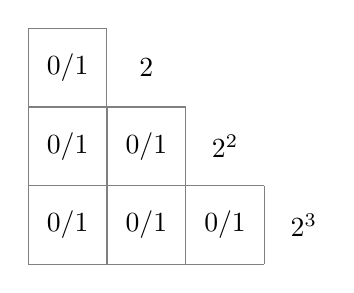
\begin{tikzpicture}
		\draw[step=1cm,gray,thin] (0, 0) grid (1,1);
		\draw[step=1cm,gray,thin] (0, 0) grid (2, -1);
		\draw[step=1cm,gray,thin] (0, -1) grid (3,-2);
		\node at (0.5,0.5) {0/1};
		\node at (1.5, 0.5) {$2$};
		\node at (0.5,-0.5) {0/1};
		\node at (1.5,-0.5) {0/1};
		\node at (2.5,-0.5) {$2^2$};
		\node at (0.5,-1.5) {0/1};
		\node at (1.5,-1.5) {0/1};
		\node at (2.5,-1.5) {0/1};
		\node at (3.5,-1.5) {$2^3$};
	\end{tikzpicture}
	\end{figure}	
	给定三个空位所能包含的信息单元总数为:$2+2^2+2^3 = 14$。 我们知道十进制是满10进一个位,二进制则是满2进一个空位。
	\begin{lstlisting}
comper(32, 2)  # 8589934590
comper(64, 2)  # 36893488147419103230
comper(32, 4)  # 24595658764946068820
comper(64, 4)  # 453709822561251284617832809909024281940
\end{lstlisting}
\end{frame}


\begin{frame}{课前预习题目浅析}
排列组合题目(捆绑法): 
\begin{figure}[H]
		\centering
		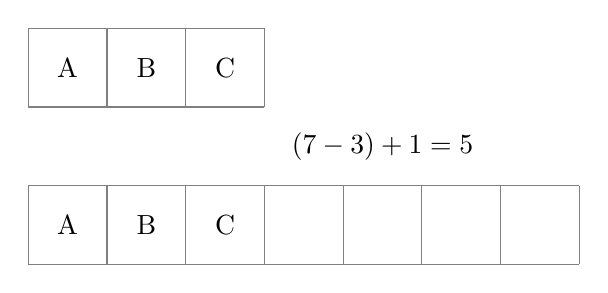
\begin{tikzpicture}
		\draw[step=1cm,gray,thin] (0, 0) grid (3, 1);
		\node at (0.5,0.5) {A};
		\node at (1.5,0.5) {B};
		\node at (2.5,0.5) {C};
		\node at (4.5, -0.5) {$(7-3)+1 = 5$};
		\node at (0.5,-1.5) {A};
		\node at (1.5,-1.5) {B};
		\node at (2.5,-1.5) {C};
		\draw[step=1cm, gray, thin] (0, -1) grid (7, -2);
	\end{tikzpicture}
	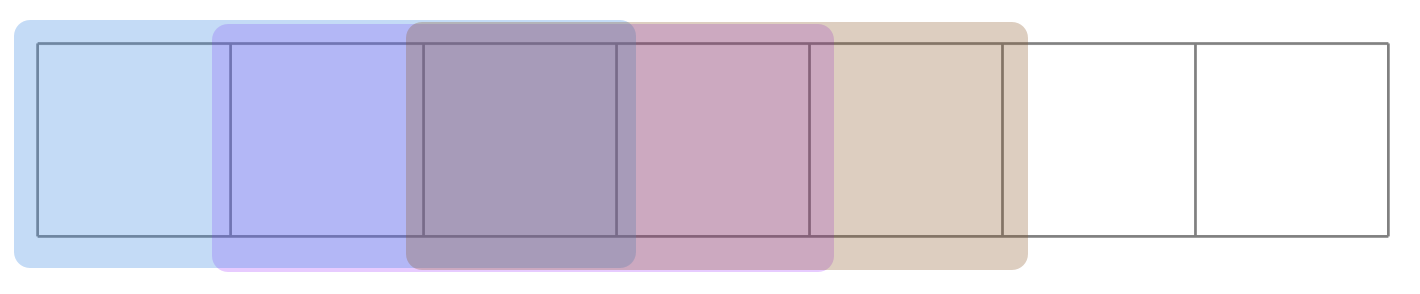
\includegraphics[width=0.61\textwidth]{fig/permutation}
	\end{figure}	
	给定参数向量$A$长度为$m$, 数据向量$B$长度为$n$, 其中$n> m$, 我们共有的排列组合方式:$n-m+1$
\end{frame}

\begin{frame}{课前预习题目浅析}
排列组合题目(捆绑法): 
\begin{columns}
	\begin{column}{0.5\textwidth}
	\begin{figure}[H]
		\centering
		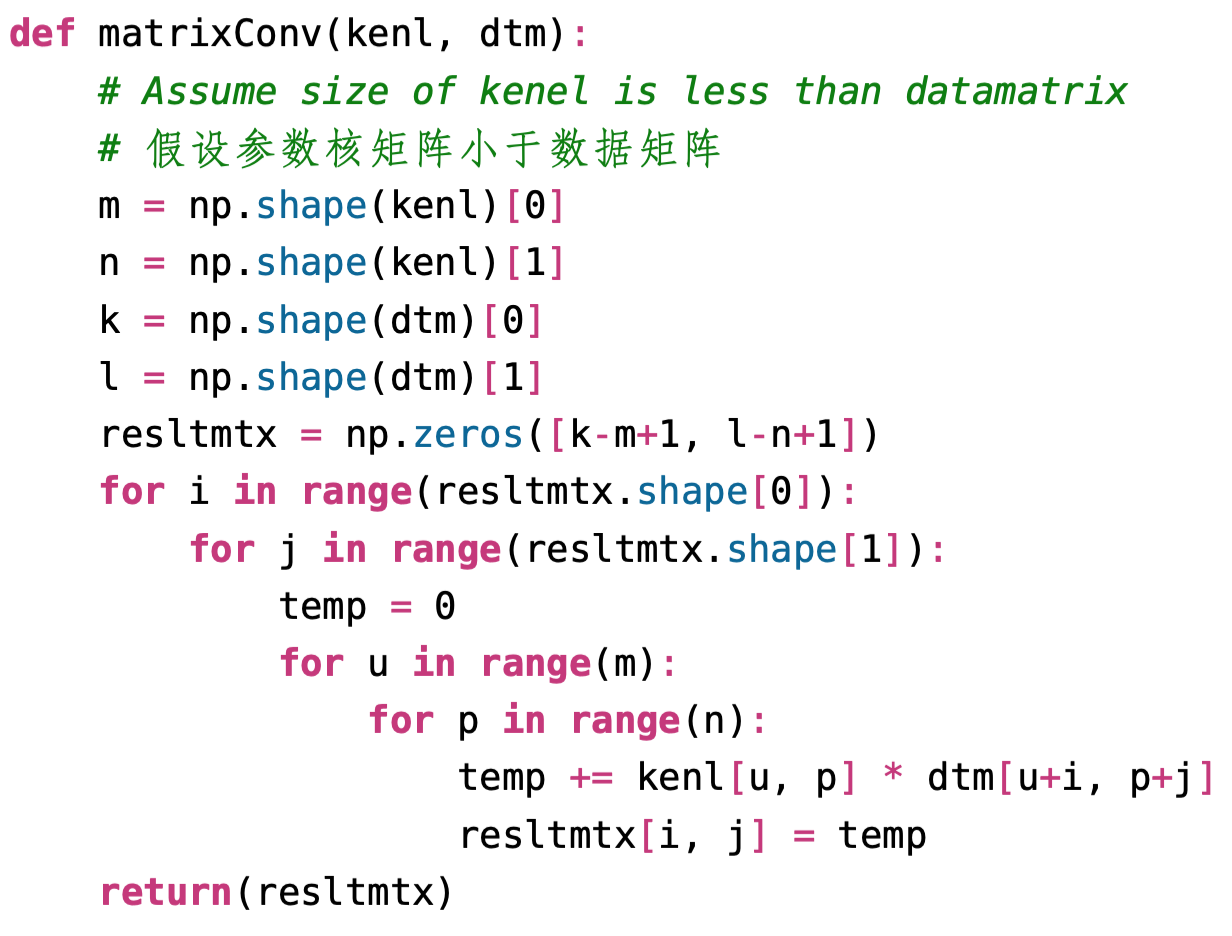
\includegraphics[width=0.96\textwidth]{fig/covfun}
	\end{figure}
	\end{column}
	\begin{column}{0.5\textwidth}
	\begin{figure}[H]
		\centering
		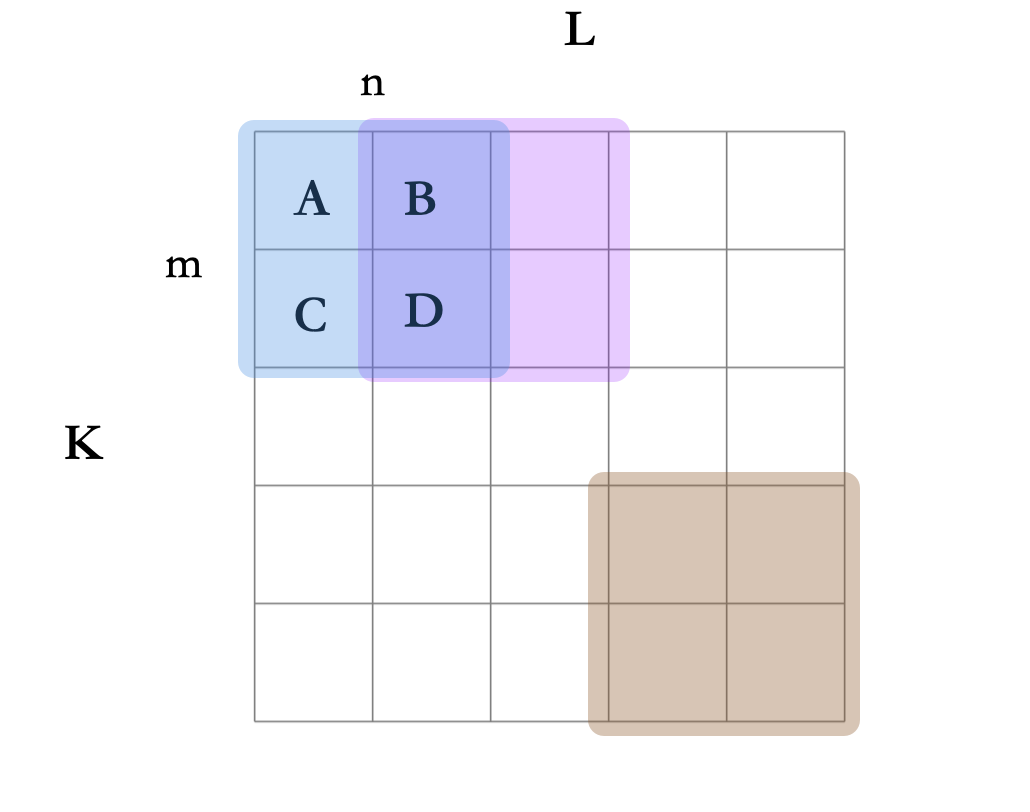
\includegraphics[width=0.99\textwidth]{fig/permatrix}
	\end{figure}	
	\end{column}
\end{columns}

给定参数核矩阵$\mathbb{A}$, 大小为$m \times n$, 数据矩阵$\mathbb{B}$,大小为$K \times L$, 其中$K >m, L> n$, 我们可以得到的结果矩阵大小为$(K-m+1) \times (L-n+1)$。
\end{frame}

\begin{frame}{三色图结构}
任何颜色都可以有红绿蓝(R, G, B)三色来调和构成:
\begin{columns}
	\begin{column}{0.35\textwidth}
		\begin{itemize}
			\item \underline{图像维度} 
			\item \footnotesize{$(1104, 1600, 3)$}
			\item \underline{注意右图的坐标}
			\item 为什么彩虹只有七色?
			\item 数字游戏:
			\item C(3, 2) = 6 + 3 = 9 = 7+2 
		\end{itemize}
	\end{column}
	\begin{column}{0.65\textwidth}
		\begin{figure}[H]
	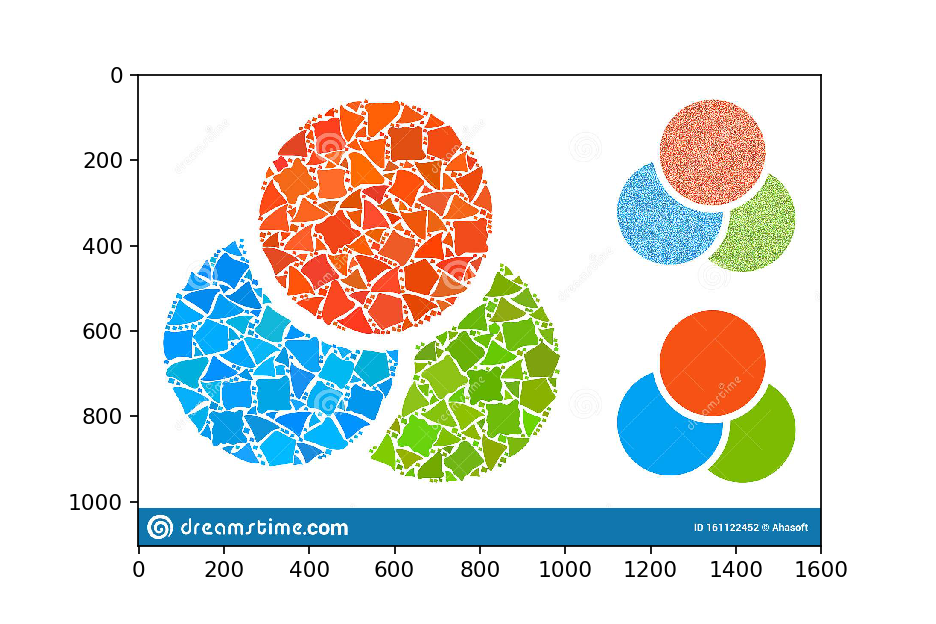
\includegraphics[width=\textwidth, right]{/Users/Michael/Documents/MDLforBeginners/Chapter3/Notes/fig/rgbmosaic.png}
\end{figure}	
	\end{column}
\end{columns}
\end{frame}

\begin{frame}{三色图结构}
	如何成为一个马赛克绘画艺术家?
	\begin{figure}[H]
		\centering
		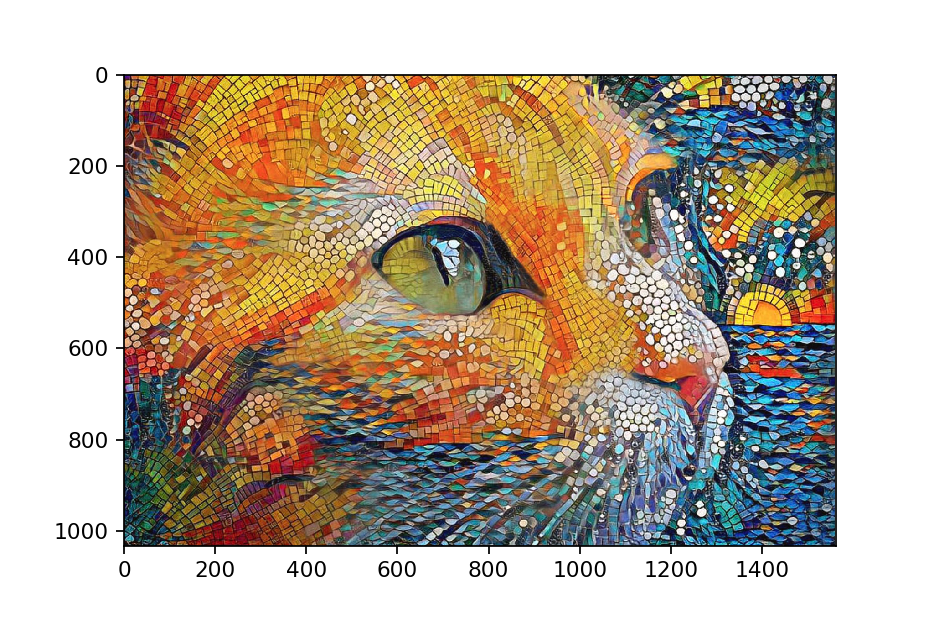
\includegraphics[width=0.96\textwidth]{/Users/Michael/Documents/MDLforBeginners/Chapter3/Notes/fig/catmosaic.png}
	\end{figure}
\end{frame}

\begin{frame}{三色图结构}
红-255, 绿-255, 蓝-255; 数值大小表示颜色`浓度’。
\begin{columns}
	\begin{column}{0.35\textwidth}
		\begin{itemize}
			\item \footnotesize{图像维度 $(1104, 1600, 3)$}
			\item $(500:520, 600:620, 0)$
			\item $(500:520, 600:620, 1)$
			\item $(500:520, 600:620, 2)$
			\item $(500:520, 230:250, 0)$
			\item $(500:520, 230:250, 1)$
			\item $(500:520, 230:250, 2)$
		\end{itemize}
	\end{column}
	\begin{column}{0.65\textwidth}
		\begin{figure}[H]
	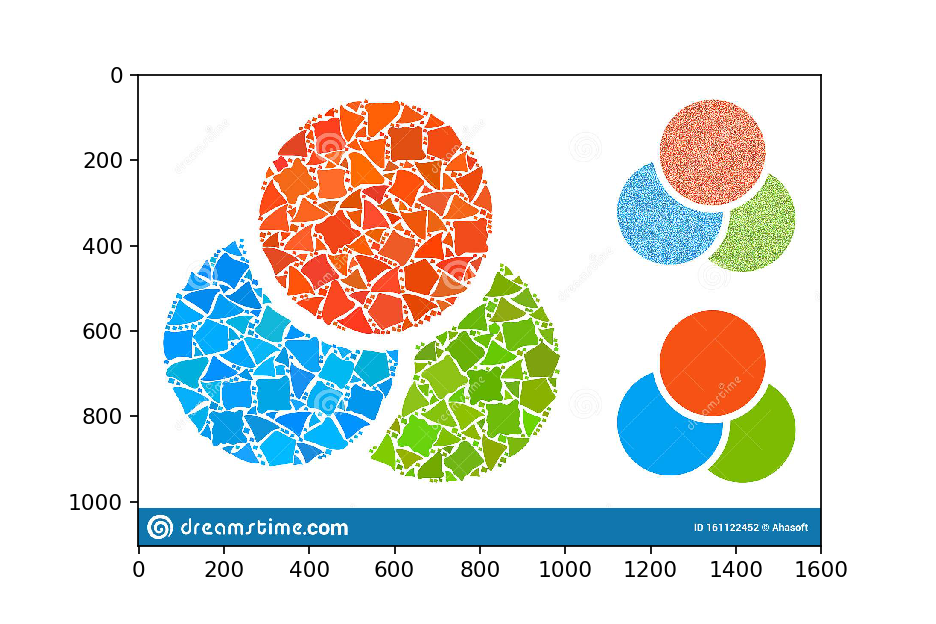
\includegraphics[width=\textwidth, right]{/Users/Michael/Documents/MDLforBeginners/Chapter3/Notes/fig/rgbmosaic.png}
\end{figure}	
	\end{column}
\end{columns}
\end{frame}

\begin{frame}{三色图结构}
\begin{figure}[H]
	\centering
	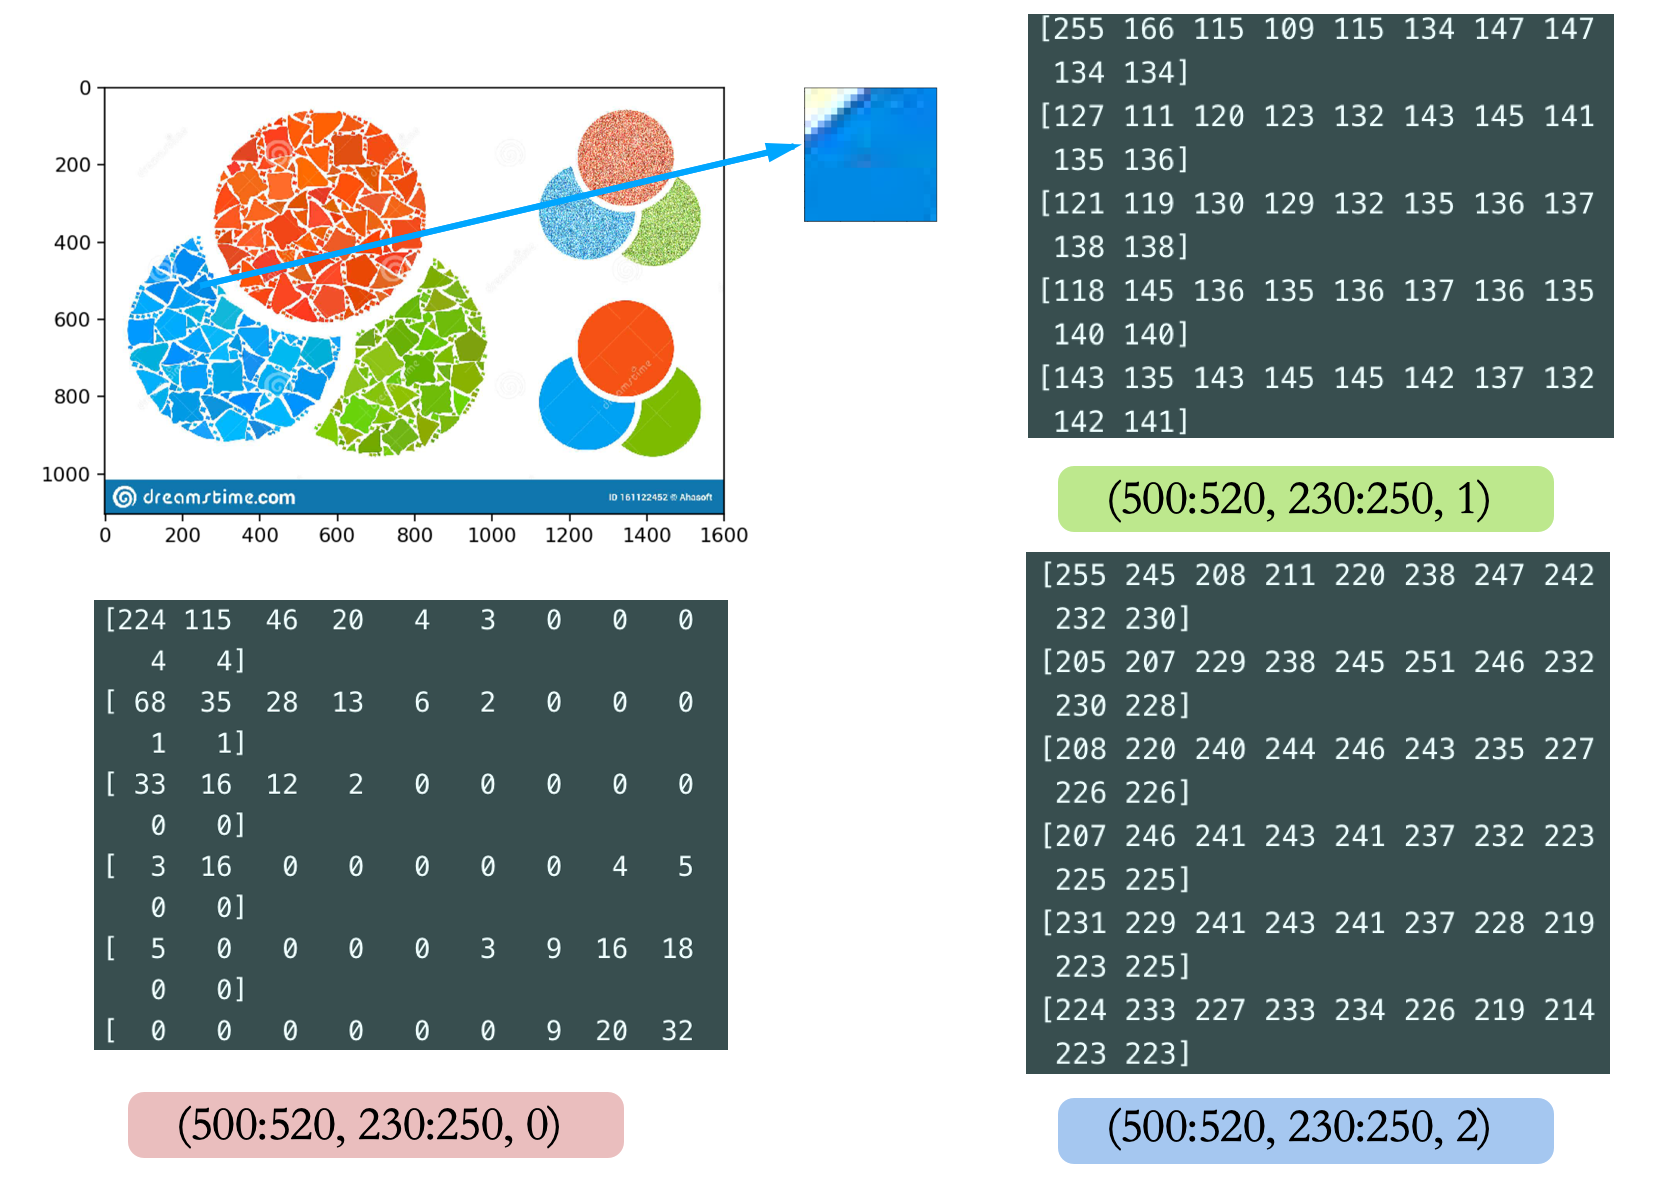
\includegraphics[width=0.9\textwidth]{fig/rgbdecomposition}
\end{figure}
\end{frame}


\section{人工智能的思维方式}

\begin{frame}{学习过程的一般性原理}
	\begin{figure}[H]
		\centering
		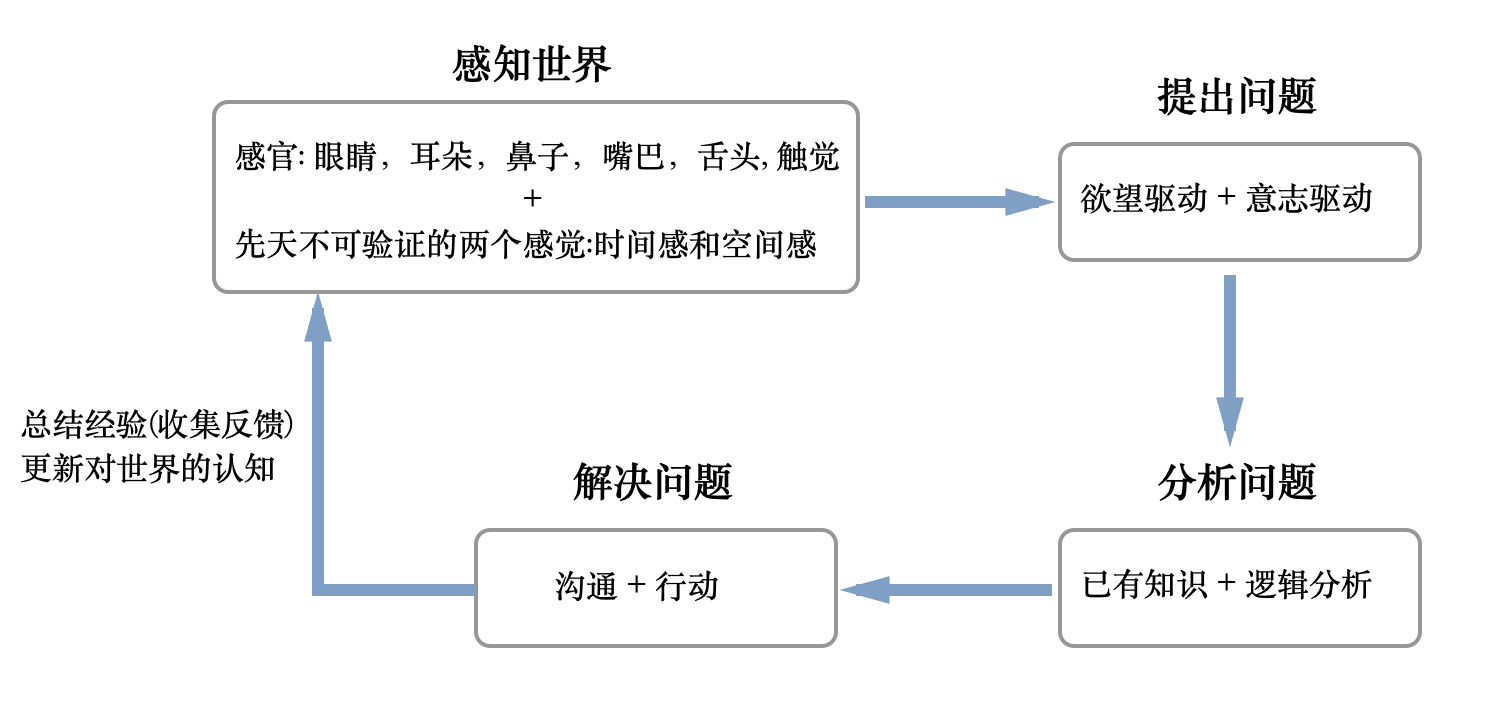
\includegraphics[width=0.99\textwidth]{/Users/Michael/Documents/MDLforBeginners/Chapter3/Notes/fig/epismeflow.png}
	\end{figure}
\end{frame}

\begin{frame}{人工智能取代人?}
	\begin{itemize}
		\item 需求端(demand): 我要,我要,我就要 
		\item 供求端(supply): 我能,我能,我很能 
	\end{itemize}
\begin{columns}
	\begin{column}{0.5\textwidth}
		\begin{figure}[H]
			\centering
			\includegraphics[width=\textwidth]{fig/circketinsect}
		\end{figure}
	\end{column}
	\begin{column}{0.5\textwidth}
			\begin{figure}[H]
		\centering
		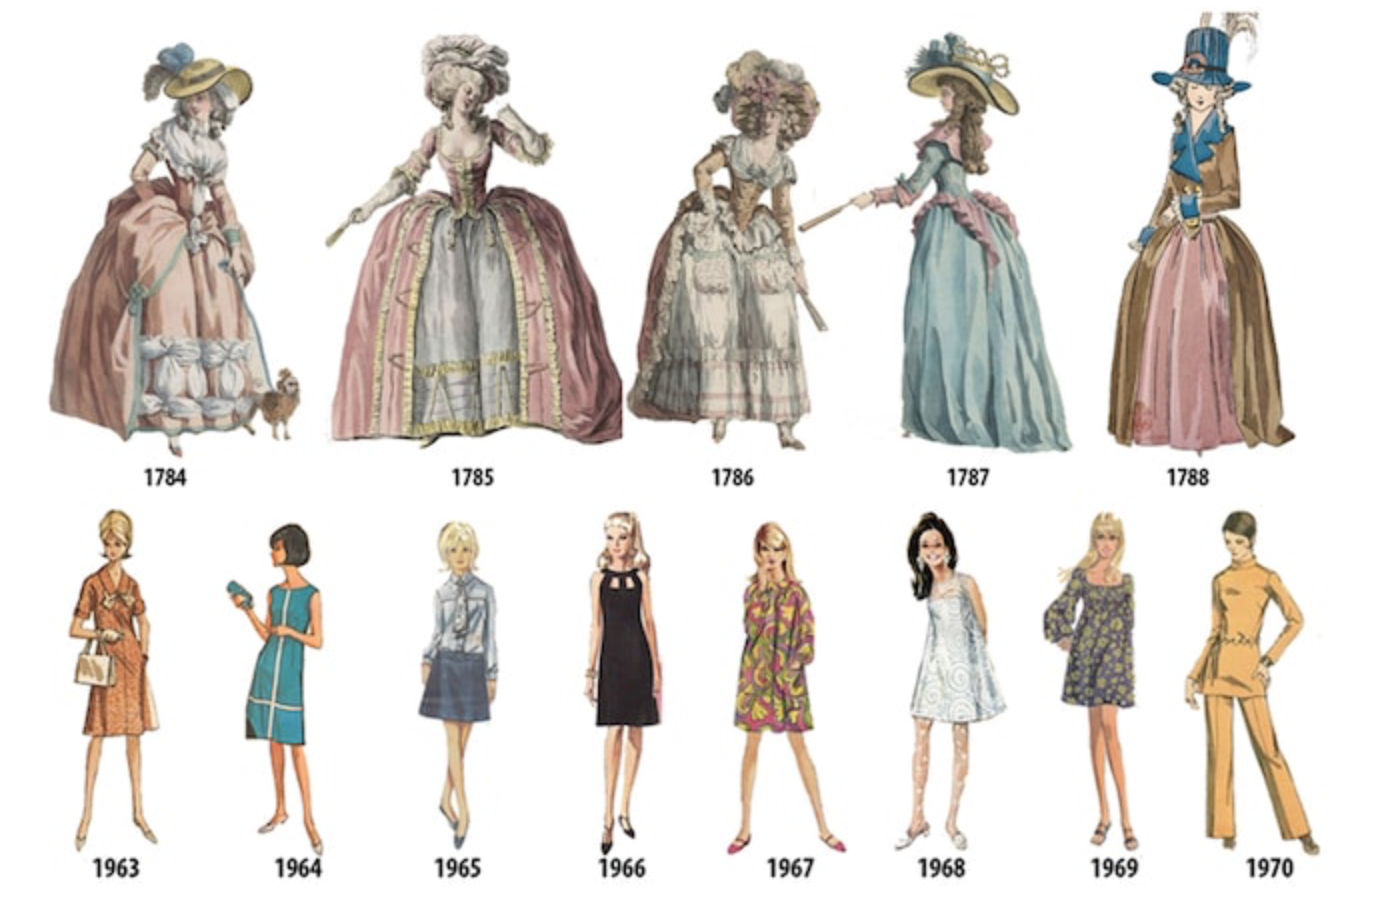
\includegraphics[width=\textwidth]{fig/fashionevolv}
	\end{figure}
	\end{column}
\end{columns}
\end{frame}

\begin{frame}{读点历史没坏处}
	\begin{itemize}
		\item 需求端(demand): 我要,我要,我就要 (1949-1979)
		\item 供求端(supply): 我能,我能,我很能 (1979-2009)
		\item 70\% 服务业(13亿工程师和全民皆兵的区别? e.g. 二战前的德国)
		\item 文官治国(所以军队是得配个政委的)
	\end{itemize}
\begin{columns}
	\begin{column}{0.5\textwidth}
		\begin{figure}[H]
			\centering
			\includegraphics[width=\textwidth]{fig/circketinsect}
		\end{figure}
	\end{column}
	\begin{column}{0.5\textwidth}
			\begin{figure}[H]
		\centering
		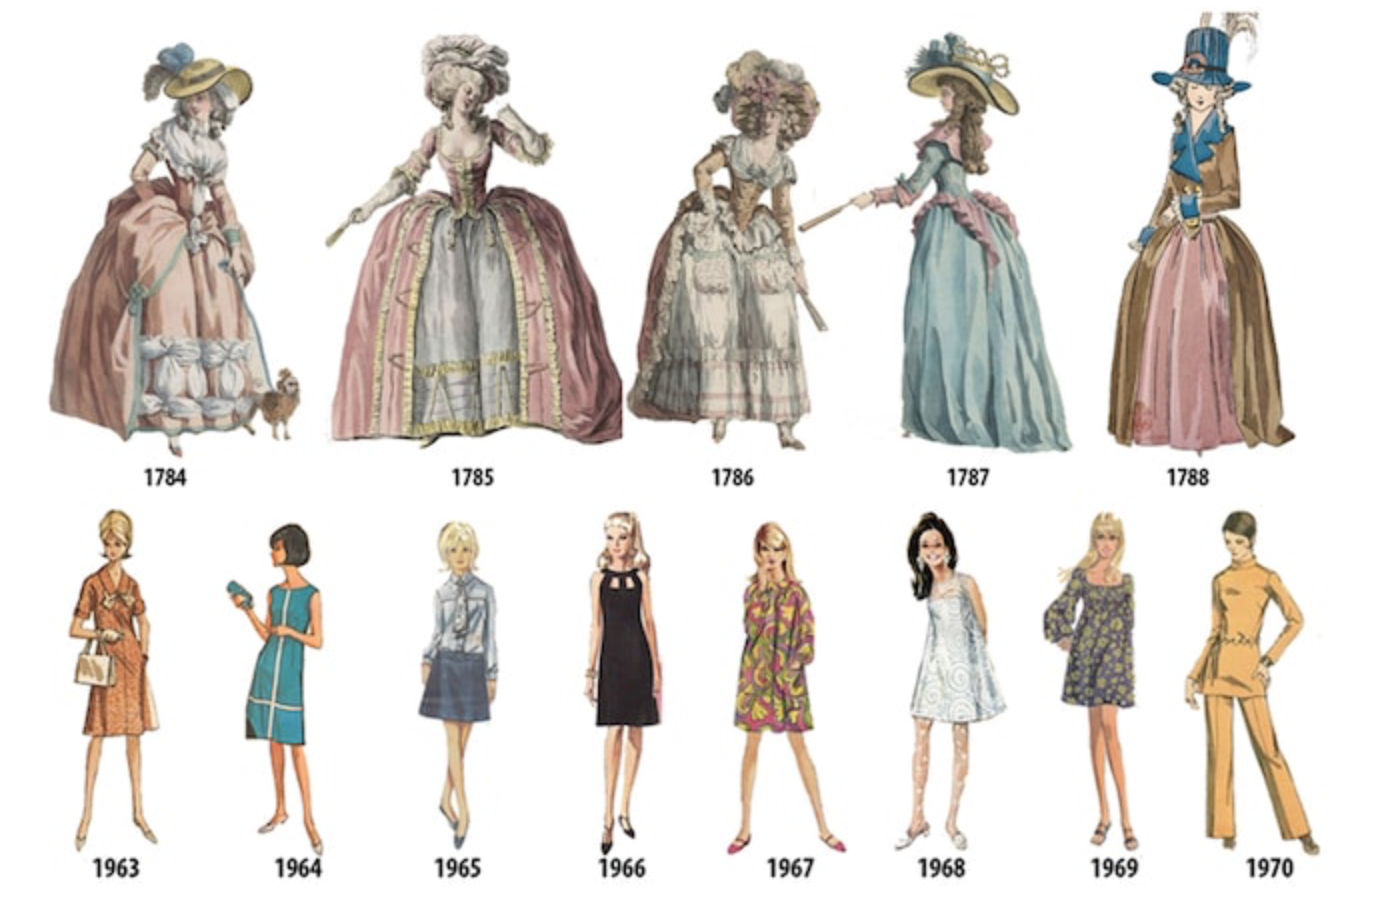
\includegraphics[width=\textwidth]{fig/fashionevolv}
	\end{figure}
	\end{column}
\end{columns}
\end{frame}

\begin{frame}{人工智能的思维方式}

传统的问题解决方式和人工智能问题解决方式最大的不同体现在以下两个方面:
	\begin{itemize}
	\setlength\itemsep{1em}
		\item 传统的问题解决方式着重对问题进行分步骤拆解和处理;
		\item 人工智能对问题的解决方式着重对整个流程的\underline{两个端口}进行数据和模型调试。
	\end{itemize}	
\end{frame}

\begin{frame}{人工智能的思维方式}
教材中有两张图片,即图3-15和图3-19,给出了神经网络模型的工作流程。我们把两个图片中的模型进行简化,绘制下面这张流程图(来源:斯坦福大学深度学习官网)。
\begin{figure}[H]
	\centering
	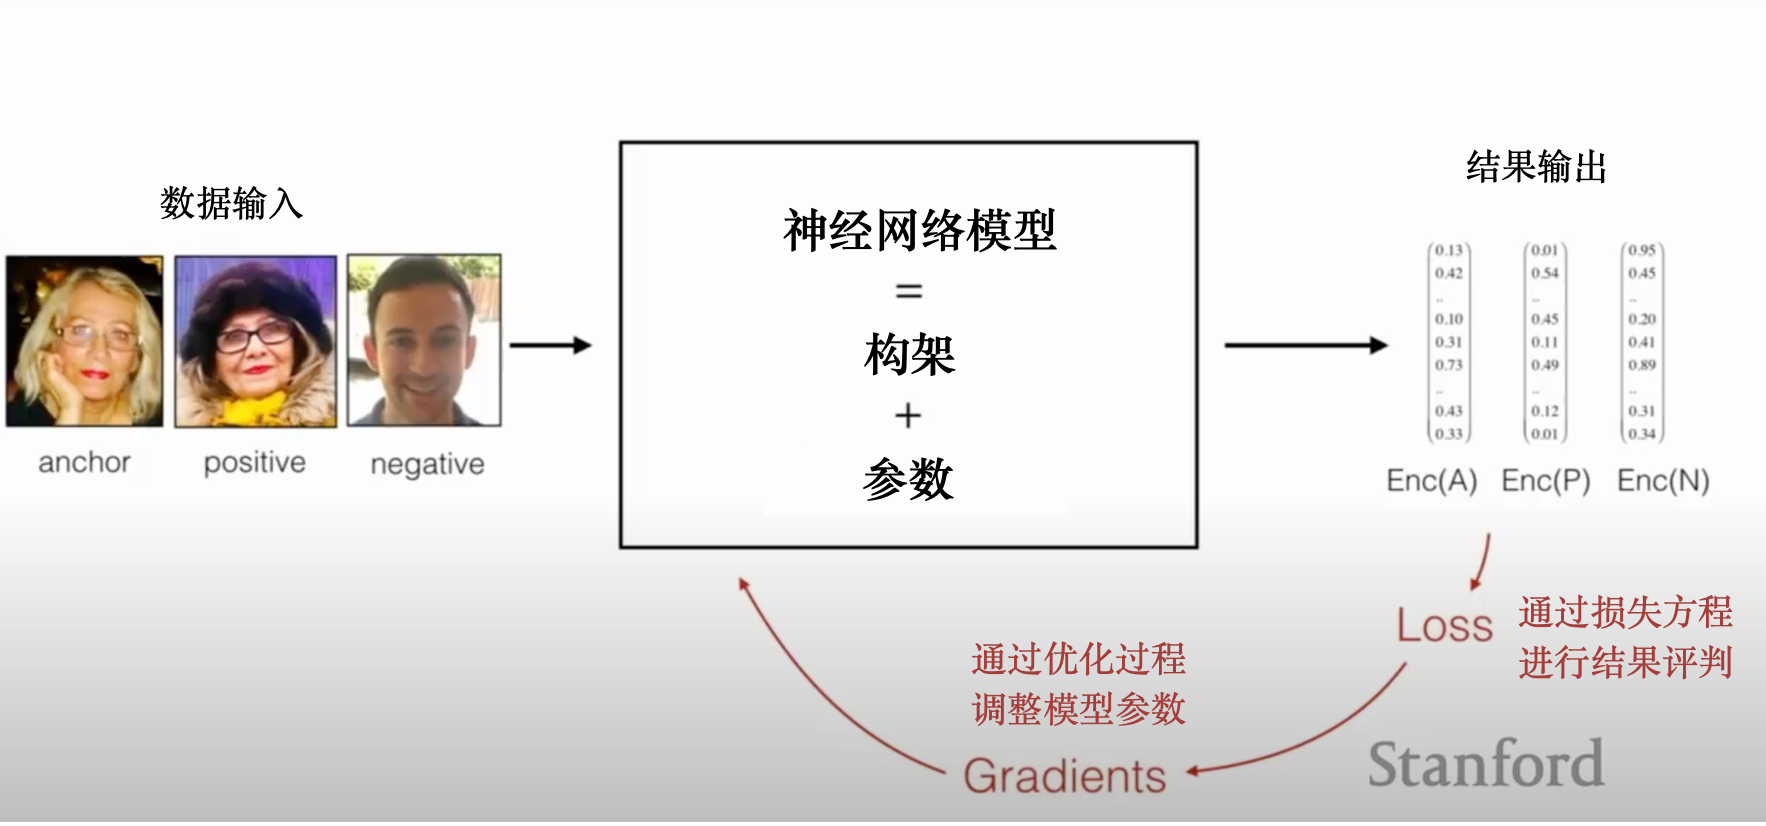
\includegraphics[width=0.99\textwidth]{/Users/Michael/Documents/MDLforBeginners/Chapter3/Notes/fig/deepmindflow.png}
\end{figure}
\end{frame}

\begin{frame}{深度神经网络模型}
	概念的关联(神经网络): 构加 + 参数
	\begin{figure}[H]
		\centering
		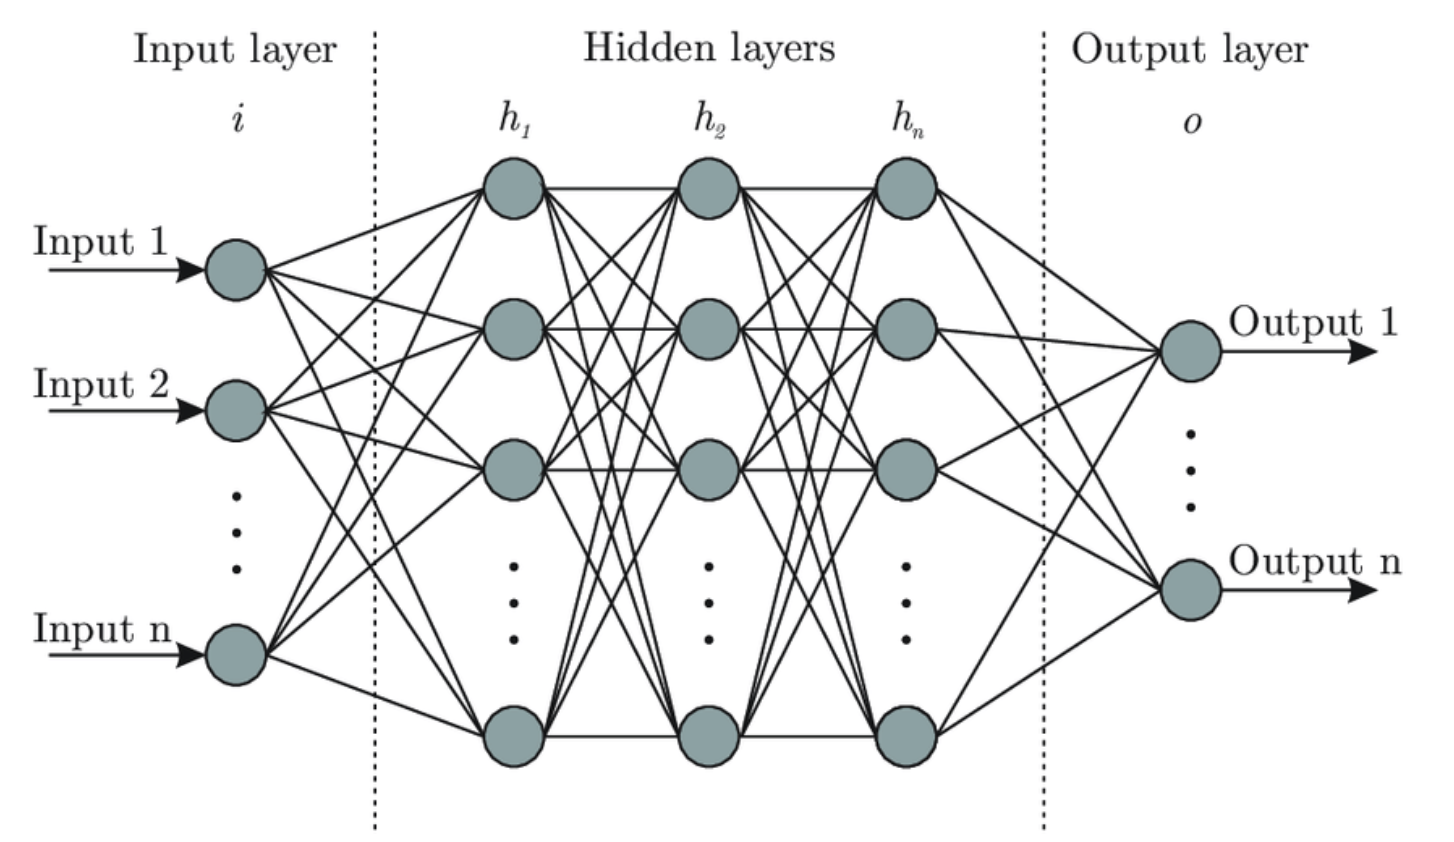
\includegraphics[width=0.8\textwidth]{fig/StdNN}
	\end{figure}
\end{frame}

\begin{frame}{人工智能思维方式:数据石油}
	为什么是深度神经网络;为什么数据是未来的石油?
	\begin{figure}[H]
		\centering
		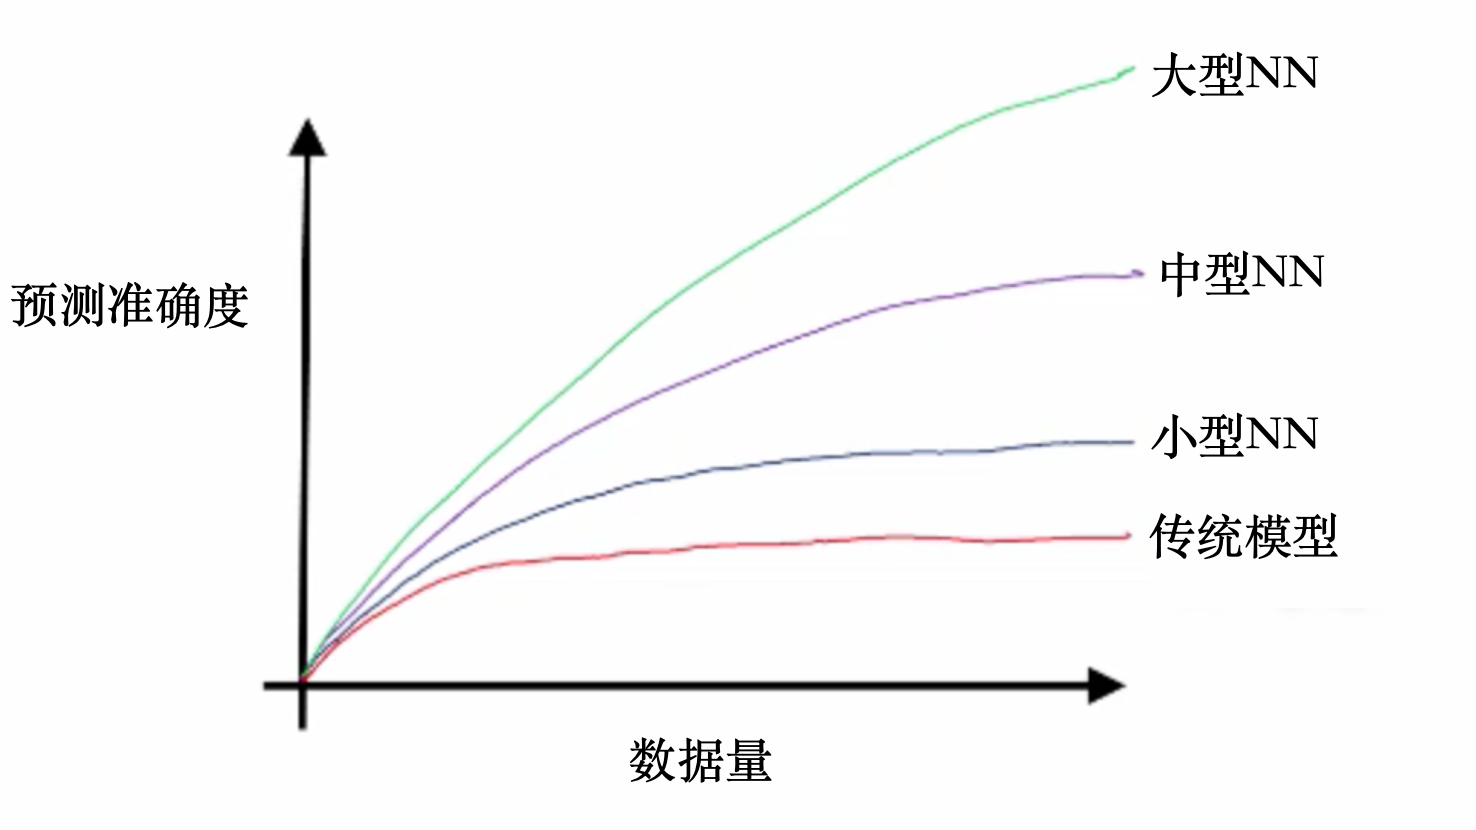
\includegraphics[width=0.9\textwidth]{fig/dataoil}
		\caption{数据量和模型表现关系(Andrew, NG, 2018)}
	\end{figure}
\end{frame}

%		\begin{tikzpicture}
%\begin{axis}[
%  ticks = none,
%  samples=100,
%  ymax=3,
%  axis x line=bottom,axis y line=left,xlabel={数据量}, ylabel={模型表现}
%]
%\addplot[cyan,domain=0.001:30, line width=0.35mm,
%restrict y to domain=0:16] {log2(x+1)};
%\addplot[red!70!black,domain=-2:1.4] {exp(x)};
%
%\node[pin={90:$f(x)=\lvert\log x\rvert$},inner sep=0pt] 
%  at (axis cs:{2,log10(2)}) {};
%\node[pin={0:$f(x)=e^{x}$},inner sep=0pt] 
%  at (axis cs:{1,exp(1)}) {};
%\end{axis}
%\end{tikzpicture}

\begin{frame}{人工智能的思维方式}
机器学习(人工智能): \textbf{通过对输入端的数据群(大数据)进行标注和整理后,建立一个人工智能构架,并设定目标函数(损失方程),对所建立的构建(或模型)进行反复训练,直到找到符合我们目标函数要求的参数核矩阵。}
\begin{figure}[H]
	\centering
	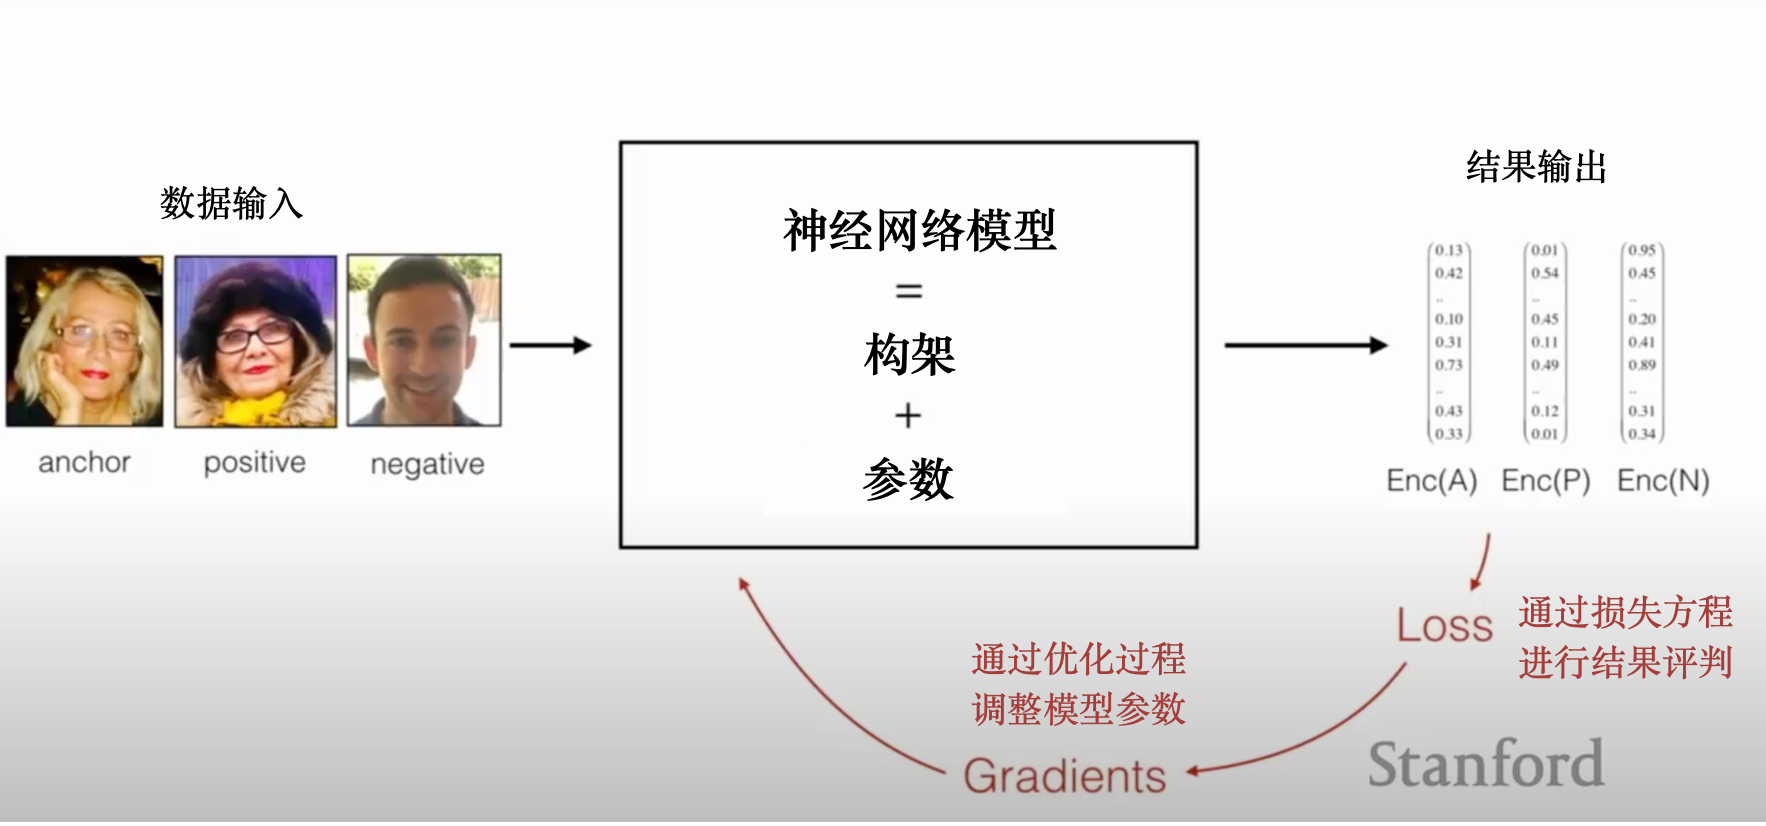
\includegraphics[width=0.9\textwidth]{/Users/Michael/Documents/MDLforBeginners/Chapter3/Notes/fig/deepmindflow.png}
\end{figure}
\end{frame}


\section{数据结构}


\setbeamercolor{block title alerted}{use=structure,fg=white,bg=structure.fg!75!black}
\setbeamercolor{block body alerted}{parent=normal text,use=block title,bg=block title.bg!10!bg}

\begin{frame}{数据结构定义}
	因为机器学习和人工智能需要大量的数据,所以非常有必要对数据结构进行定义和分类。 生活中最常见的数据形式应该是Excel表格。
	\begin{definition}
	我们把由数字和对其的描述(有其根据)组成的信息形态,称为\textit{数据};我们将统一在一个描述下的数列,称为\text{数据集}; 有多个数据集构成的一系列数据,称为\textit{数据阵}。
\end{definition}
\begin{figure}[H]
	\centering
	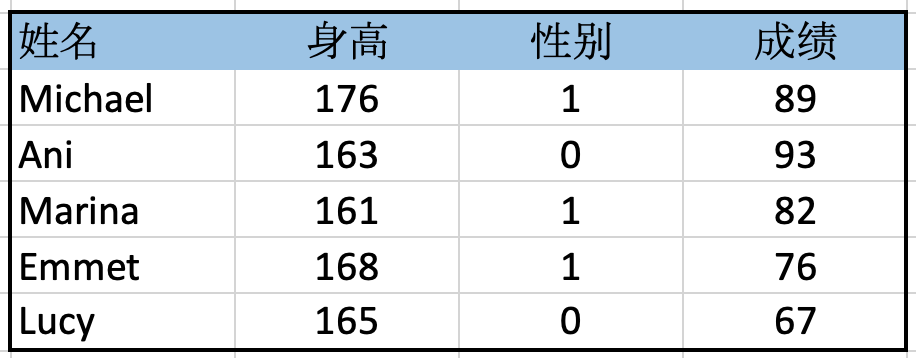
\includegraphics[width=0.67\textwidth]{/Users/Michael/Documents/MDLforBeginners/Chapter3/Notes/fig/dataframeEx.png}
\end{figure}
\end{frame}


\begin{frame}{数据结构定义}
\begin{definition}
	我们把语言文本,网页信息,图片和影音等的复合数据,称为\textit{多媒体数据集}。
\end{definition}

\begin{definition}
	我们将多媒体数据集和数据阵组合构成的数据形态成为\textit{数据群}或者\textit{大数据}。数据群或大数据,在业界也被称为\textbf{有标注的数据群}。
\end{definition}
比如,下面这个数据群,就是一个有标注的数据群。
{\footnotesize
\begin{table}[H]
	\centering
	\renewcommand{\arraystretch}{1.5}
	\begin{tabular}{ccccc}
	\hline 
		图片(1400, 1400, 3) & 年份 & 地点 & 备注1 & 备注2 \\
		\hline 
		图1 & 2016 & 桥 & 青岛 & 红色 \\
		图2 & 2020 &  伦敦 & 人 & 女 \\
		图3 & 2013 & 成都& 熊猫 & 国宝\\
		\hline 
	\end{tabular}
\end{table}
}
\end{frame}

\begin{frame}{数据结构定义}
多数情况下,机器学习需要有\underline{标注的数据群(大数据)}。模型的训练和数据的质量存在正相关关系。
\begin{figure}[H]
	\centering
	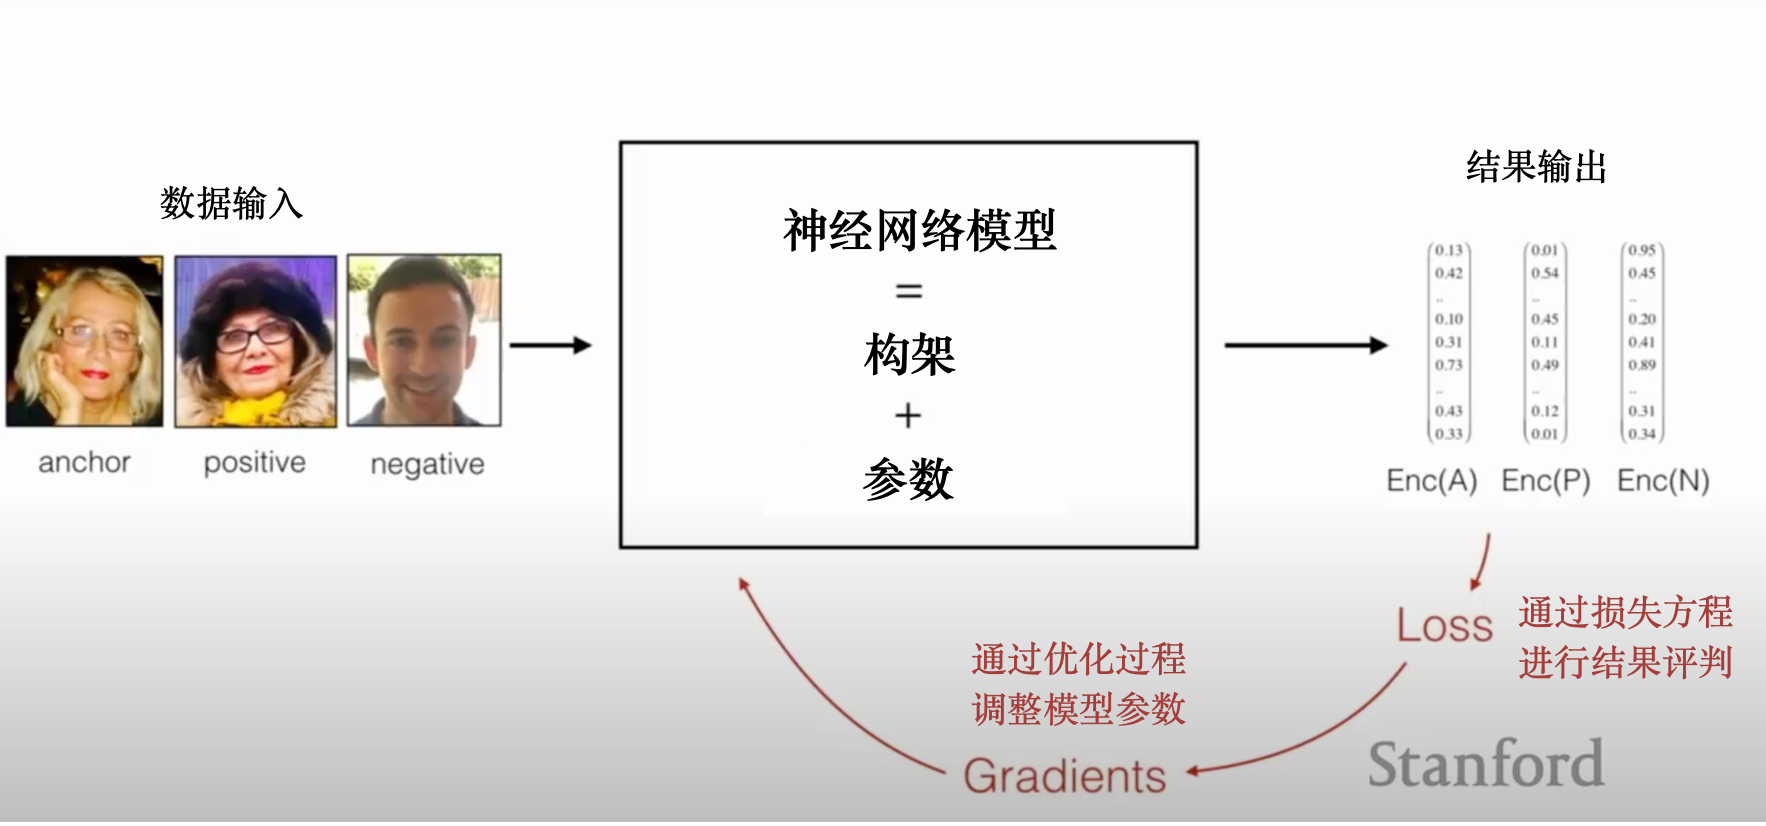
\includegraphics[width=0.99\textwidth]{/Users/Michael/Documents/MDLforBeginners/Chapter3/Notes/fig/deepmindflow.png}
\end{figure}
\end{frame}


\section{损失方程(Loss Function)}

\begin{frame}{损失方程}
拥有了标注的数据,就有了\underline{对比依据}\footnote[frame]{对,没有对比就没有伤害。}, 就可以训练人工智能模型,从而可以调整模型参数,来提升预测准确度。而用来衡量准确度的方程就需要损失方程。

\hfil

\begin{definition}
	假设数据群标注过的数据准确可靠,在人工智能模型中,模型在整合输入数据且加工计算后输出的结果与数据群标注的数据差别的方程称为\textit{损失方程(Loss Function)}。损失方程的一般形式为:
\begin{align*}
	L: (Y, \hat{Y}): \ \to \rn 
\end{align*}	
\end{definition}
\end{frame}

\begin{frame}{损失方程}
比如我们想要通过人工智能来判定图片中人类的性别,下面的表格中给出了最为简单的一种损失方程。
\begin{table}[H]
	\centering
	\renewcommand{\arraystretch}{1.5}
	\begin{tabular}{cccc}
	\hline 
		图片(1400, 1400, 3) & 标注(1-男,0-女) & 模型预测 & 差异\\
		\hline 
		图1 & 1 & 0 & 1 \\
		图2 & 0 & 1 & 1 \\
		图3 & 1 & 1 & 0 \\
		\hline 
	\end{tabular}
\end{table}
用$\hat{Y}$来代表预测的结果,$Y$来代表标注结果,那么损失方程为:
\begin{align*}
	L(Y, \hat{Y}): |Y-\hat{Y}| 
\end{align*}
\end{frame}



\section{向量,矩阵的相关运算}

\begin{frame}{向量和矩阵}
无论是\textit{多媒体数据集}还是\textit{数据阵},除去其标注的信息,具体的数都是储存在矩阵中的。
\begin{definition}
	\textit{矩阵}(Matrix)是一个按照长方阵列排列的复数或实数集合。对一个矩阵的简单描述可以为 $m \times n$ 的矩阵,即该矩阵有$m$ 行,$n$列. $m \times n$也被称为矩阵的大小。
\end{definition}
\begin{example}
比如,我们有$3 \times 3 $的矩阵$A$ 和$2 \times 3$ 的矩阵$B$。
\begin{align*}
	 A = \begin{bmatrix}
	1 & 3 & 4 \\
	2 & 5 & 8 \\
	3 & 9 & 7
\end{bmatrix}, & & B = \begin{bmatrix}
	3.2 & 1.9 & 5.7 \\
	4.1 & 5.8 & 9.3 \\
\end{bmatrix}
\end{align*}	
\end{example}
\end{frame}

\begin{frame}{向量和矩阵}
\begin{definition}
	矩阵中单独的一行被成为\textit{行向量}(row vector), 单独的一列别成为\textit{列向量}(column vector)。
\end{definition}
\begin{example}
比如在上面的矩阵$A$中,	我们有以下单独的向量:
\begin{align*}
	A_{r2} = [2 \ 5 \ 8],  & & A_{c2} = \begin{bmatrix}
		3 \\
		5 \\
		9 
	\end{bmatrix}
\end{align*}
\end{example}
\end{frame}

\begin{frame}{矩阵运算}
\begin{definition}
	现有同样大小的$m \times n$的矩阵 $A, B$, 我们定义矩阵的加法($+$)运算为:
	\begin{align*}
		A + B = \begin{bmatrix}
			(a_{11} + b_{11}) & (a_{12}+b_{12}) & \cdots & (a_{1n}+b_{1n}) \\
			a_{21} + b_{21} & a_{22}+b_{22} & \cdots & a_{2n}+b_{2n} \\
			\vdots & \ddots & & \vdots \\
			a_{m1} + b_{m1} & a_{m2}+b_{m2} & \cdots & a_{mn}+b_{mn} \\
		\end{bmatrix}
	\end{align*}
	其中,$a_{ij}$ 为矩阵$A$中第$i$行第$j$列元素,$b_{ij}$ 为矩阵$B$中第$i$行第$j$列元素。
\end{definition}

注意: 矩阵的加法只能在同样大小的矩阵中进行,即同位元素相加。	

\end{frame}

\begin{frame}{矩阵运算}
矩阵最早的提出是为了解决多项式的求解,比如下面方程组的转换。
\begin{align*}
	2x_1 + 3x_2 + 7x_3 & = 9 \\
	4x_1 + 5x_2 + 8 x_3 & = 10 \\
	\begin{bmatrix}
		2 & 3 & 7 \\
		4 & 5 & 8 
	\end{bmatrix} \begin{bmatrix}
		x_1 \\
		x_2 \\
		x_3 
	\end{bmatrix} & = \begin{bmatrix}
		 9 \\
		 10 
	\end{bmatrix}
\end{align*}

\begin{definition}
	现有$m \times n$ 的矩阵A 和 $n \times k$的矩阵$B$, 我们定义矩阵的乘法$\cdot$为
	\begin{align*}
		(A \cdot B)_{ij} = \sum_{r=1}^n a_{ir}b_{rj} = a_{i1}b_{1j} + a_{i2}b_{2j} + \cdots + a_{in}b_{nj}
	\end{align*}
	其中$(A \dot B)_{ij}$是两个矩阵相乘后的第i行第j列元素。
\end{definition}	
\end{frame}

\begin{frame}{矩阵运算}
注意: 取任意$a \times b$ 矩阵A 和$c \times d$ 矩阵 B, 如果$b \neq c$,则两个矩阵不可以相乘。	

\hfil 

\begin{example}
计算下列矩阵的乘法
\begin{align*}
	\begin{bmatrix}
		2 & 3 & 7 \\
		4 & 5 & 8 
	\end{bmatrix} \begin{bmatrix}
		1 \\
		0 \\
		-1 
	\end{bmatrix} = \ ? & & \begin{bmatrix}
		1 & 3 & 3 \\
		2 & 8 & 4 \\
		3 & 9 & 1 
	\end{bmatrix} \begin{bmatrix}
		3 & 2 \\
		1 & 0 \\
		-1 & 8 
	\end{bmatrix} = \ ?
\end{align*}	
\end{example}
\end{frame}


\section{卷积运算(Convolution)}


\begin{frame}{卷积(Convolution)}
卷积运算(Convolution)是图形处理中特有的一种运算方式。其目的是\textbf{系统性一次性得}对原始图片进行快速处理。我们之前已经讲解过图形的储存形式,而且在课前预习中的习题中也特别对卷积运算进行了铺垫,接下来我们就更加规范得对这个概念进行学习。
\end{frame}


\begin{frame}{向量卷积(Vector Convolution)}
\begin{definition}
{\footnotesize
	给定一个长度为$m$的向量$A$和一个长度为$n$的向量$B$, 其中$n > m$:
	\begin{align*}
		A & = [a_1, a_2, \cdots, a_m ] \\
		B & = [b_1, b_2, \cdots, \cdots, a_n]
	\end{align*}
	我们称$A$为\textit{参数(核)向量}(kernel vector),$B$为\textit{数据向量},其卷积运算(convolution)$*$定义为
\begin{algorithm}[H]
	\SetAlgoLined
	\caption{Convolution Operation}
	初始化长度为$n-m+1$的向量$C = [c_1, c_2, \cdots, c_{n-m+1}]$ \;
	$C = A * B $ \; 其中,每一个元素的计算方法为\;
	\For {$i \ in \ [1:n-m+1]$}{$c_i = \sum_{k=1}^m a_k b_{k+i-1} = a_1 b_i +  a_2 b_{i+1} +\cdots + a_m b_{i+m-1}$}
	\end{algorithm}
}
\end{definition}
\end{frame}

\begin{frame}{向量卷积(Vector Convolution)}
\begin{example}
	现有参数向量$A=[1, 3, 4]$ 和数据向量$B = [5, 6, 7 , 8 , 9]$,那么
	\begin{align*}
		A * B & = [34, 40, 46]\\
		34 & = 1\times 5 + 3 \times 6 + 4 \times 7 \\
		40 & = 1 \times 6 + 3 \times 7 + 4 \times 8 
	\end{align*}
\end{example}
\end{frame}


\begin{frame}{矩阵卷积(Matrix Convolution)}
\begin{definition}
	给定一个$m \times n$的矩阵$A$,和一个$k \times l$的矩阵$B$,并且$k > m, l > n$, 那么矩阵$A$被叫作\textit{参数(核)矩阵}(kernel matrix),矩阵$B$被称为\textit{数据矩阵}。那么矩阵$A$和$B$的卷积运算定义为
	\begin{align*}
		A * B = \text{移动参数向量对数据向量进行对位求积后求和}
	\end{align*}
	运算过程如下图所示(来源:Irhum Shafkat, 2018)。
\end{definition}
矩阵的卷积有很多种,更多的介绍请参考该网站:

\url{https://towardsdatascience.com/intuitively-understanding-convolutions-for-deep-learning-1f6f42faee1}。
\end{frame}

\begin{frame}{矩阵卷积(Matrix Convolution)}
\begin{figure}[H]
	\centering
	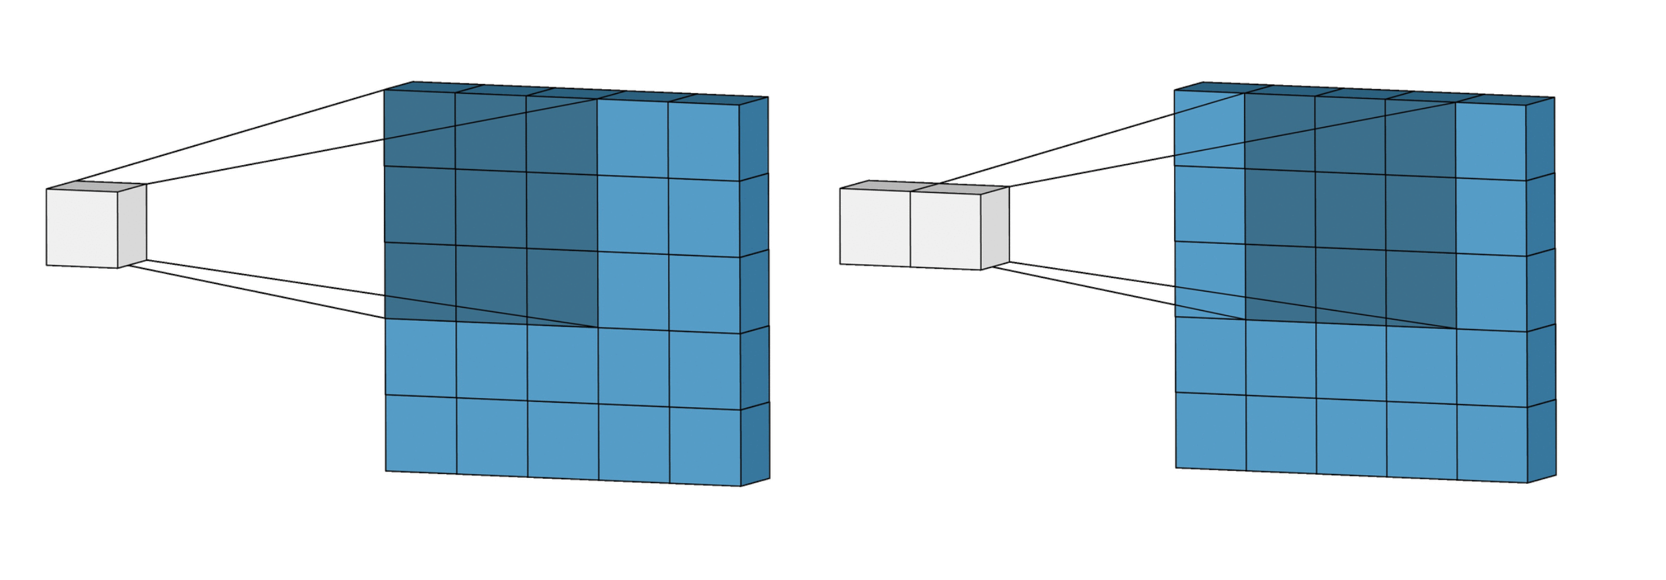
\includegraphics[width=\textwidth]{/Users/Michael/Documents/MDLforBeginners/Chapter3/Notes/fig/mtconvo.png}
	\caption{矩阵卷积演示(Irhum Shafkat, 2018)}
\end{figure}
\end{frame}

\begin{frame}{矩阵卷积(Matrix Convolution)}
矩阵的卷积运算目的是想要通过参数矩阵来对数据矩阵进行进一步的处理。之所以需要这个处理过程是因为
	\begin{itemize}
	\setlength\itemsep{1em}
		\item 原始多媒体数据集维数较大,比如图3.4中的猫有$(1400, 1400, 3)$,即$1400 \times 1400 \times 3 = 588000$个数(元素)组成。通过卷积运算后数据集的维数会有所下降,从而节省模型训练时间;
		\item 原始多媒体数据集的特征不明显,需要通过参数矩阵的卷积运算后来进行优化;
		\item 卷积在图像识别中的应用原因还有其它的,以后我们会结合具体案例进一步讲解。卷积运算主要应用在图像识别中,在其它领域,比如金融数据的人工智能模型,则没有被那么广泛得使用
	\end{itemize}
\end{frame}

\begin{frame}{矩阵卷积(Matrix Convolution)}
\begin{example}
{\footnotesize
我们手动计算一种标准的卷积形式,给定参数核矩阵$A$和数据矩阵$B$为
\begin{align*}
	A = \begin{bmatrix}
		1 & -1 \\
		1 & 2 
	\end{bmatrix} & & B= \begin{bmatrix}
		1 & 2 & 1 \\
		2 & 3 & 6 \\
		0 & 5 & 7 
	\end{bmatrix}
\end{align*}	
$C=A*B$的最终结果为\begin{align*}
	C = \begin{bmatrix}
		7 & 16 \\
		9 & 16 
	\end{bmatrix}
\end{align*} 你会发现$C$中元素最大值是$14$,刚好在$B$的右下角。
我们演示计算结果矩阵($C = A*B$)的第一个元素:
\begin{align*}
	C_{11} = 1\times 1 + (-1) \times 2 + 1 \times 2 + 2 \times 3 = 7 
\end{align*}
}
\end{example}
\end{frame}


\begin{frame}{卷积案例}
下面的表格是一个班级内几名同学的不同学科的成绩表,我们来计算不同的参数卷积矩阵可以给出不同的`评估'结果(这个评估结果可以理解成我们机器学习的一个运算结果)。
\begin{figure}[H]
	\centering
	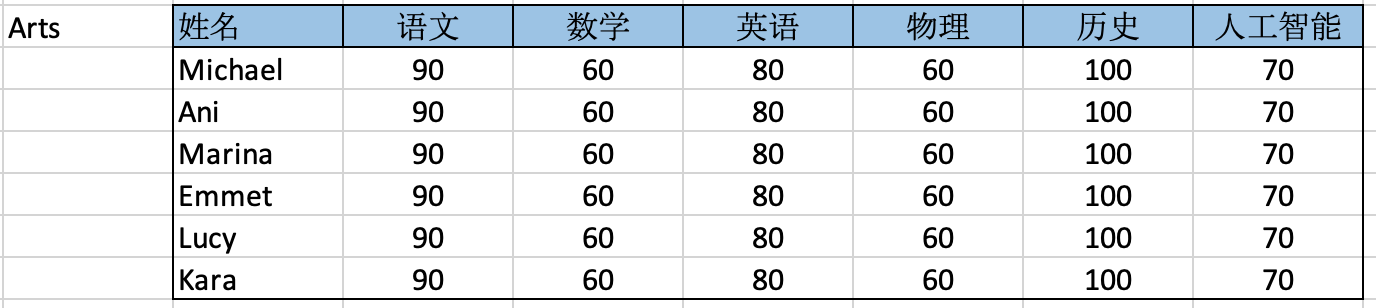
\includegraphics[width=\textwidth]{/Users/Michael/Documents/MDLforBeginners/Chapter3/Notes/fig/artsgrade.png}
	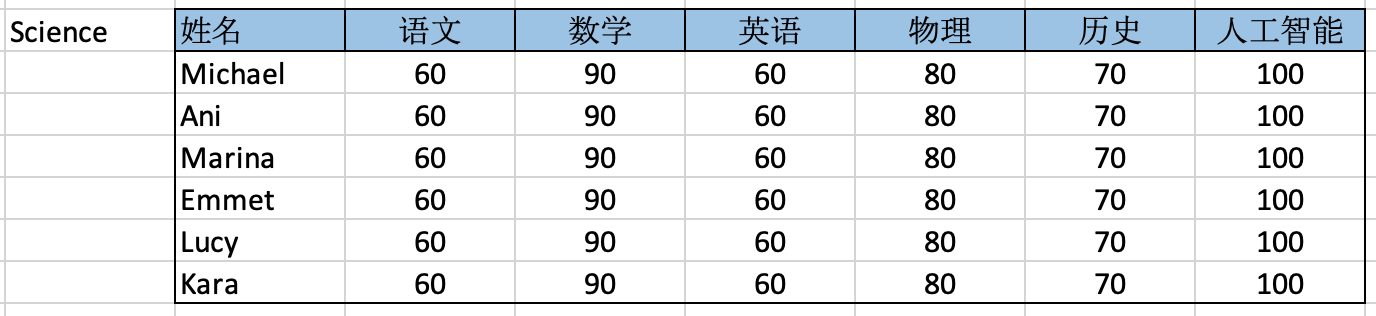
\includegraphics[width=\textwidth]{/Users/Michael/Documents/MDLforBeginners/Chapter3/Notes/fig/sciencegrade.png}
\end{figure}
\end{frame}

\begin{frame}{卷积案例}
其中参数核(kernel)矩阵给定为
\begin{align*}
	K = \begin{bmatrix}
		1 & 0 & $-$1$$ \\
		1 & 0 & $-$1$$  \\
		1 & 0 & $-$1$$  
	\end{bmatrix}
\end{align*}
将文科生(arts)和理科生(science)的数据阵进行两次卷积运算:
{\footnotesize
\begin{align*}
	A \Rightarrow \begin{bmatrix}
		30 &    0  &   -60  &    -30 \\
       30  &     0  &    -60  &    -30   \\        
       30  &     0  &    -60  &   -30 \\
       30  &    0  &    -60  &   -30 
	\end{bmatrix} \Rightarrow \begin{bmatrix}
		270 & 90 \\
		270 & 90 
	\end{bmatrix} & & 	S \Rightarrow \begin{bmatrix}
	   0 & 30 & -30 & -60 \\
       0 & 30 &  -30 & -60 \\
        0 & 30 &  -30 & -60 \\
       0 & 30 &  -30 &  -60
	\end{bmatrix} \Rightarrow \begin{bmatrix}
		90 & 270 \\
		90 & 270 
	\end{bmatrix}
\end{align*}
}
两个矩阵看起来很相似,只是列向量顺序不同。
\end{frame}

\begin{frame}{卷积案例}
如果我们将两个矩阵按照此前的顺序进行标注,可以得出下面的表格:
\begin{table}[H]
\renewcommand{\arraystretch}{1.2}
	\centering
	\begin{tabular}{|l|cc|}
	\hline 
		学生/成绩集成 & 文科成绩 & 理科成绩 \\
		\hline 
		文科生& 270 & 90 \\
		& 270 & 90 \\
		\hline 
		理科生& 90 & 270 \\
		& 90 & 270 \\
		\hline 
	\end{tabular}
\end{table}
{\footnotesize
复杂神经学习模型要比以上的例子复杂的多,但是基本流程却非常相似,具体的计算和演化逻辑也可以说`如出一辙'。我们可以把神经网络深度学习的模型再一次概况为:\textbf{通过对输入端的数据群(大数据)进行标注和整理后,建立一个人工智能构架,并设定目标函数(损失方程),对所建立的构建(或模型)进行反复训练,直到找到符合我们目标函数要求的参数核矩阵。}
}
\end{frame}


\begin{frame}{再见}
	Thank you !  请完成课后习题C3 !
\begin{columns}
	\begin{column}{0.4\textwidth}
			\begin{figure}[H]
				\centering
			
\includegraphics[width=\textwidth]{/Users/Michael/Documents/MDLforBeginners/Chapter3/Notes/fig/C3C1qrcode.png}
			\caption{C3C1-问卷}
			\end{figure}
	\end{column}
	\begin{column}{0.4\textwidth}
		\begin{figure}[H]
	
\includegraphics[width=\textwidth]{/Users/Michael/Documents/MDLforBeginners/Chapter3/Notes/fig/C3C2qrcode.png}
	\caption{C3C2-问卷}
\end{figure}	
	\end{column}
\end{columns}
\end{frame}



\begin{frame}[allowframebreaks]{Reference}
  \bibliography{p3.bib}
  \bibliographystyle{apalike}
  I will add reference list later, in which only two websites should be listed. 
\end{frame}


\begin{frame}{My Vision (我的愿景)}

markets can remain irrational longer than you can remain solvent

\hfill - \textit{John Maynard Keynes}

Only when the tide goes out do you discover who's been swimming naked

\hfill - \textit{Warren Buffett }

人工智能教育:
\hfil

\begin{itemize}
\setlength\itemsep{1em}
	\item 教材 + 习题 + 案例 (Latex, markdown, HTML5, data visualisation, etc.) 
	\item 风口浪尖上的线上转线下(codecademy, 淘宝)
	\item 数学教育革新(计算机和编程的全面引入)
	\item International Summer School 
	\item 如果我成为一名父母
\end{itemize}
\end{frame}



\end{document}
